\section{Statistics of 6 networks}
In this section I will present some statistics about the 6 chosen networks. The results will be presented in tables. It is also noteworthy to reiterate that Gephi does not display nodes if their degree is 0.

\textbf{Number of nodes.} The number of nodes of each graph will be the amount of people who have at least one edge connecting them to another person.

\textbf{Number of edges.} The number of edges of each graph will be the amount of connections that exist between each person for each question.

\textbf{Edge density.} Graph density tells us how connected nodes are between each other. For undirected graphs, this metric can be calculated as
\begin{equation}
    D_{undirected} = \frac{2|E|}{|N|(|N|-1)}
    \label{equation:dir_density}
\end{equation}
and the density for directed graphs is defined as
\begin{equation}
    D_{directed} = \frac{|E|}{|N|(|N    |-1)}
    \label{equation:undir_density}
\end{equation}
where $E$ is the number of edges and $V$ is the number of nodes in the graph.

\textbf{Degree distribution.} The degree distribution of a graph allows us to grasp how deeply connected the nodes are. Figure \ref{fig:4} pictures the degree distributions for the 6 chosen networks.
\begin{figure}
    \centering
    \subfloat[\centering Network 1]{{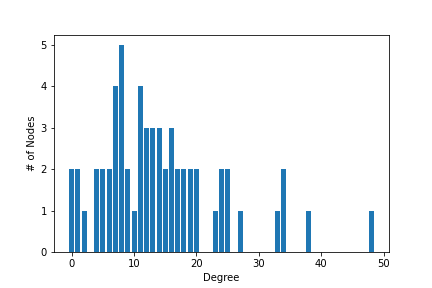
\includegraphics[width=0.45\textwidth]{img/net_0_degree_distribution.png}}}
    \qquad
    \subfloat[\centering Network 2]{{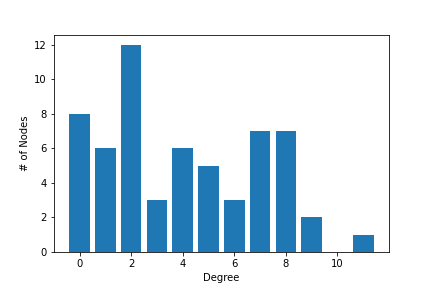
\includegraphics[width=0.45\textwidth]{img/net_1_degree_distribution.png}}}
    \qquad
    \subfloat[\centering Network 3]{{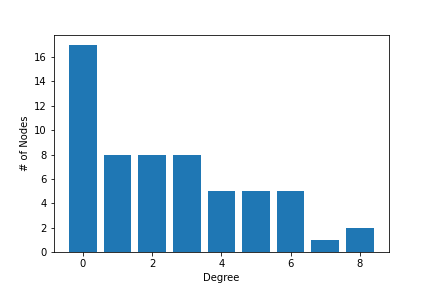
\includegraphics[width=0.45\textwidth]{img/net_2_degree_distribution.png}}}
    \qquad
    \subfloat[\centering Network 4]{{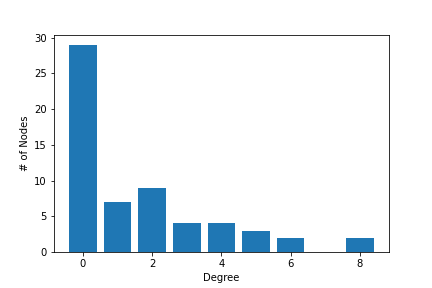
\includegraphics[width=0.45\textwidth]{img/net_3_degree_distribution.png}}}
    \qquad
    \subfloat[\centering Network 5]{{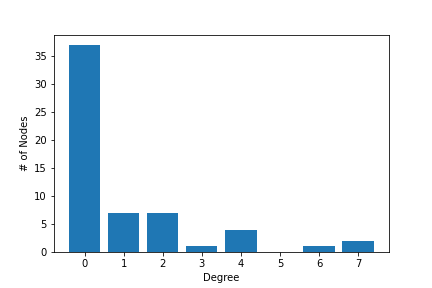
\includegraphics[width=0.45\textwidth]{img/net_4_degree_distribution.png}}}
    \qquad
    \subfloat[\centering Network 7]{{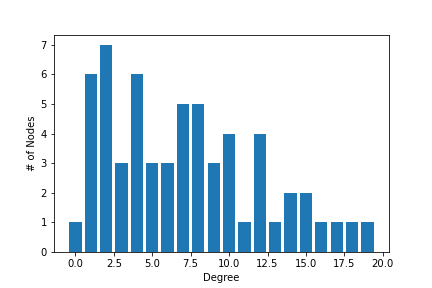
\includegraphics[width=0.45\textwidth]{img/net_6_degree_distribution.png}}}
    \caption{Degree distributions}
    \label{fig:4}
\end{figure}

\textbf{Average clustering coefficient.} The average clustering coefficient for a graph helps determine how transitive a relationship is. The clustering coefficient is defined as
\begin{equation}
    C_i = \frac{2e_i}{k_i(k_i-1)}
    \label{equation:clustering_coef}
\end{equation}
where $e_i$ is the number of edges between the neighbors of node $i$.

The average clustering coefficient of the graph is calculated as
\begin{equation}
    <C> = \frac{1}{N}\sum_{i}^{N}C_i
\end{equation}
where $N$ is the number of nodes in the graph, and $C_i$ is the clustering coefficient of node $i$.

\textbf{Number of nodes in strongly connected component (SCC).}

\textbf{Number of nodes in weakly connected component (WCC).}

\textbf{Average path length in SCC.}

\textbf{Diameter of SCC.}

\textbf{Community detection.}

\begin{table}
    \centering
    \begin{tabular}{|c|c|c|c|c|c|c|c|}
        \hline
        \textbf{Metric} & \textbf{Net. 1} & \textbf{Net. 2} & \textbf{Net. 3} & \textbf{Net. 4} & \textbf{Net. 5} & \textbf{Net. 7} \\
        \hline
        Num. Nodes & 59 & 55 & 52 & 41 & 29 & 59 \\
        \hline
        Num. Edges & 427 & 124 & 80 & 54 & 34 & 216 \\
        \hline
        Density & 0.125 & 0.084 & 0.060 & 0.066 & 0.084 & 0.126 \\
        \hline
        Avg. Clust. Coef. & 0.375 & 0.412 & 0.482 & 0.583 & 0.620 & 0.542 \\
        \hline
        Num. Nodes SCC &  &  &  &  &  &  \\
        \hline
        Num. Nodes WCC &  &  &  &  &  &  \\
        \hline
        Avg. Path Len. SCC &  &  &  &  &  &  \\
        \hline
        Diameter of SCC &  &  &  &  &  &  \\
        \hline
        Comm. Detection &  &  &  &  &  &  \\
        \hline
    \end{tabular}
    \caption{Network statistics}
    \label{table:1}
\end{table}
